\begin{frame}
	\frametitle{Allgemein}
	
\textbf{Aufgabenstellung:}

Entwickeln eines Mini-Java Compilers mit den zugehörigen Schritten: Lexer, Parser, TypChecker und Codegenerierung.
\end{frame}

\begin{frame}[fragile]
\frametitle{Allgemein - Ziel}

\textbf{Ziel} 

Korrektes Übersetzen der folgenden Klasse:

\begin{lstlisting}[language=Java]
class Fibonacci {
  int getFib(int n) {
    return (n < 2) ? n : getFib(n-1) + getFib(n-2);
  }
}
\end{lstlisting}	
\end{frame}



\begin{frame}{Allgemein - Featureliste}

Umgesetze Features (Auszug):

\pause

\begin{itemize}
	\item Ternary Operator \pause
	\item For / While / DoWhile \pause
	\item If / If-Else / Switch-Case \pause 
	\item Pre- bzw. Post Inkrement/Dekrement \pause 
	\item Arithmetische Operatoren (+, -, /, div, mod, *) inklusive Zuweisung (+=, etc.)
\end{itemize}	
\end{frame}

\begin{frame}{Allgemein - Entwicklung}

Code-Sharing über GitHub (https://github.com/Pfeifenjoy/compilerbau-WS17-18) mit continuous integration (travis).

\par \medskip

\pause

Als Build-System wird cabal eingesetzt.	
\end{frame}

\begin{frame}{Allgemein - Projektmanagement}

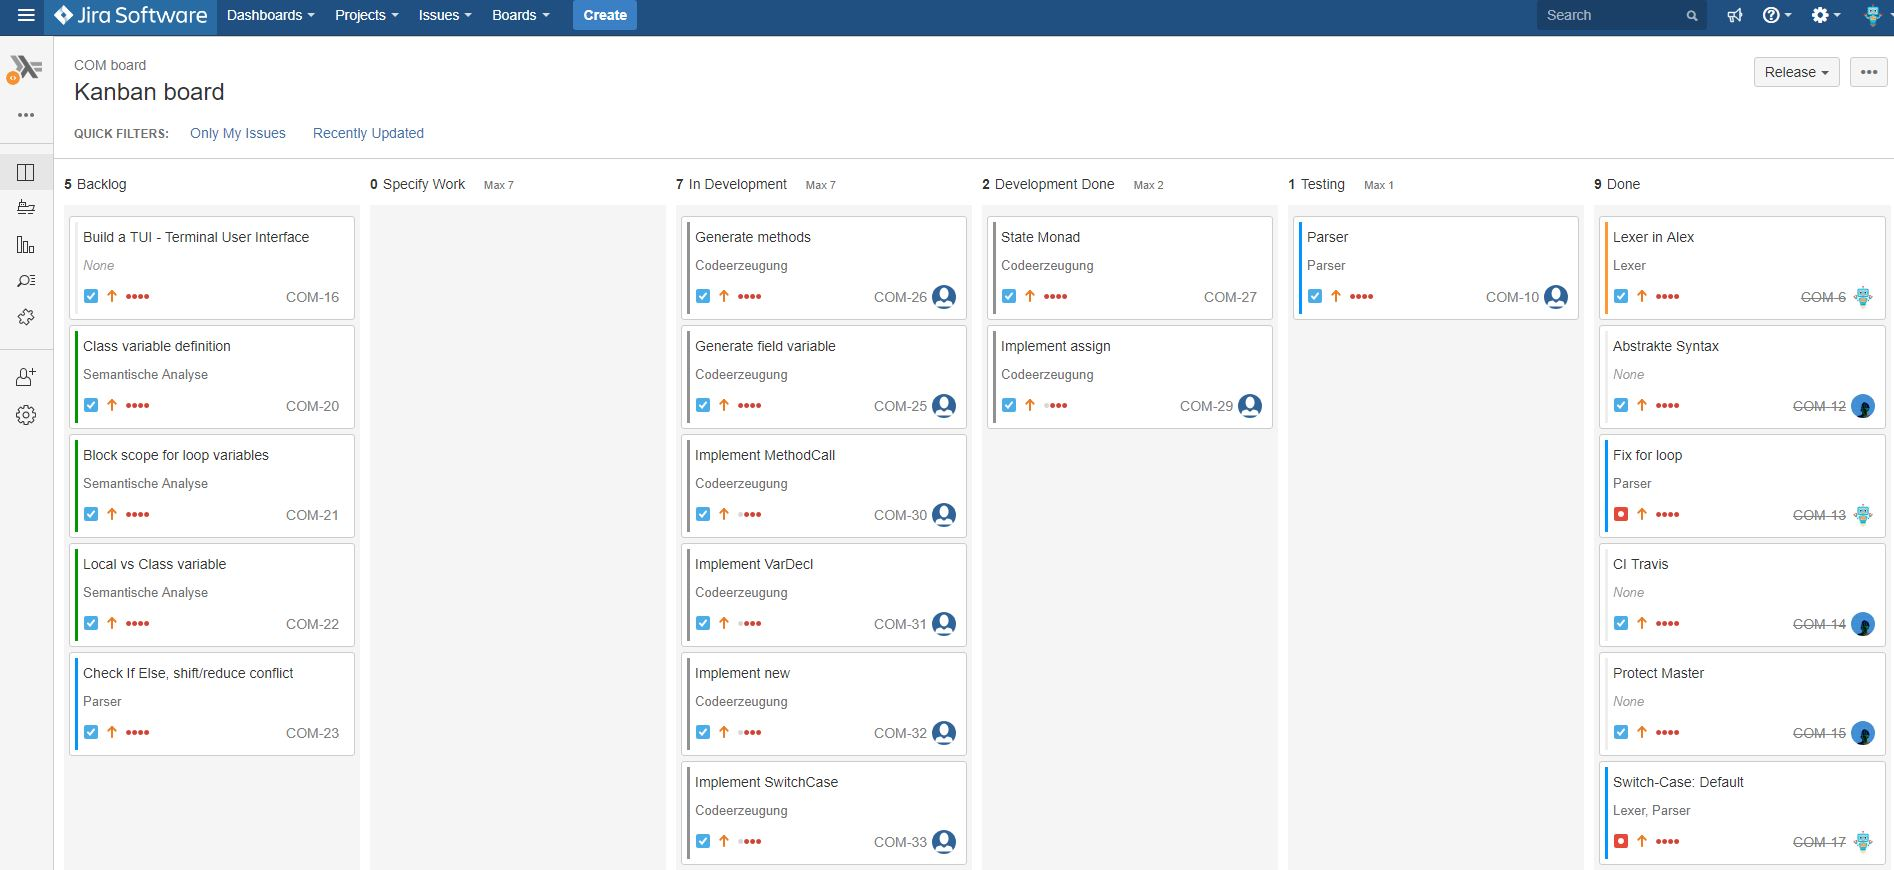
\includegraphics[scale=0.25]{images/allgemein/jira.jpg}

\end{frame}

\begin{frame}{Allgemein - JC}

\begin{itemize}
	\item Text User Interface
	\item Wechseln in Ordner: dist/build/jc
	\item Hilfe: ./jc -h
	\item Compile mit Log: ./jc File.java -l logFile
\end{itemize}

\end{frame}

\begin{frame}{Allgemein - IDE}

\begin{columns}
	\begin{column}{0.5\textwidth}
		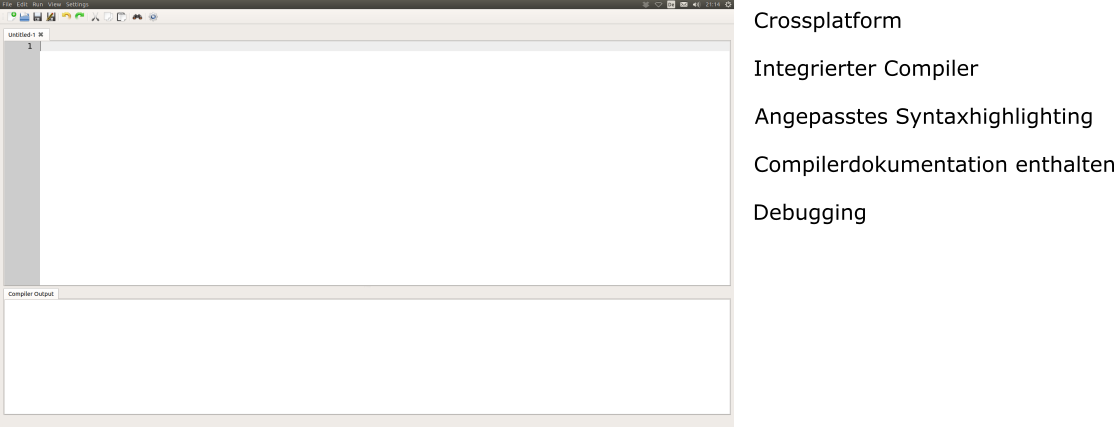
\includegraphics[scale=0.1]{images/allgemein/ide.png}
	\end{column}
	\begin{column}{0.5\textwidth}
			\begin{itemize}
				\item Python: PyQt
				\item Crossplatfrom
				\item Integrierter Compiler
				\item Angepasste Syntaxhighlighting
				\item Compilerdokumentation enthalten
				\item Debugging
			\end{itemize}
	\end{column}
\end{columns}


\end{frame}
